% -*- compile-command: "make HOCKING-peak-penalty-slides.pdf" -*-
\documentclass{beamer}
\usepackage{tikz}
\usepackage[all]{xy}
\usepackage{amsmath,amssymb}
\usepackage{hyperref}
\usepackage{graphicx}

\DeclareMathOperator*{\argmin}{arg\,min}
\DeclareMathOperator*{\Lik}{Lik}
\DeclareMathOperator*{\Peaks}{Peaks}
\DeclareMathOperator*{\Segments}{Segments}
\DeclareMathOperator*{\argmax}{arg\,max}
\DeclareMathOperator*{\maximize}{maximize}
\DeclareMathOperator*{\minimize}{minimize}
\newcommand{\sign}{\operatorname{sign}}
\newcommand{\RR}{\mathbb R}
\newcommand{\ZZ}{\mathbb Z}
\newcommand{\NN}{\mathbb N}

% Set transparency of non-highlighted sections in the table of
% contents slide.
\setbeamertemplate{section in toc shaded}[default][100]
\AtBeginSection[]
{
  \setbeamercolor{section in toc}{fg=red} 
  \setbeamercolor{section in toc shaded}{fg=black} 
  \begin{frame}
    \tableofcontents[currentsection]
  \end{frame}
}

\begin{document}

\title{PeakSeg: constrained optimal \textbf{Seg}mentation and
  supervised penalty learning for \textbf{Peak} detection in count data}

\author{
  Toby Dylan Hocking\\
  toby.hocking@mail.mcgill.ca\\
  joint work with Guillem Rigaill and Guillaume Bourque}

\date{7 July 2015}

\maketitle

\section{ChIP-seq data and previous work on peak detection}


\begin{frame}
  \frametitle{Problem: many false
    positives in unsupervised peak detectors}

  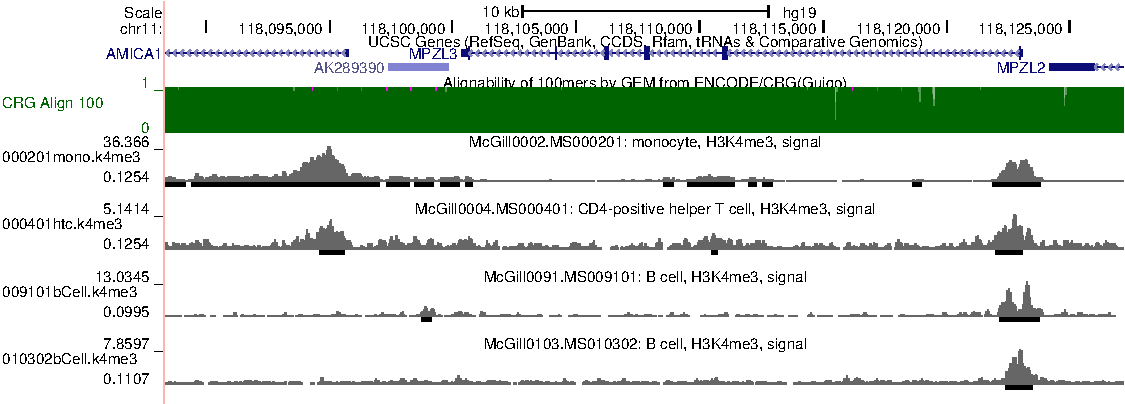
\includegraphics[width=\textwidth]{../PeakSegDP-NIPS/screenshot-ucsc-edited}

  \begin{itemize}
    \item Grey signal is noisy count data ($\approx$protein binding).
    \item Binary classification for every sample and position: \\
      negative class = background noise,\\
      positive class = ``peaks.''
    \item Black bands show peak predictions of ``Model-based analysis of
      ChIP-Seq'' (MACS), Zhang et al, 2008 (default parameters).
  \end{itemize}
\end{frame}

\begin{frame}
  \frametitle{Peak detector accuracy can be quantified using manually
    annotated region labels}
  
  \includegraphics[width=1.1\textwidth]{figure-good-bad}

  \begin{itemize}
  \item Good peaks have 0 incorrect regions.
  \item Bad peaks have 7 incorrect regions.
  \item Goal: minimize number of incorrect test labels.
  \end{itemize}

\end{frame}

\section{New PeakSeg model: constrained optimal segmentation}

\begin{frame}
  \frametitle{Maximum likelihood Poisson segmentation models}
  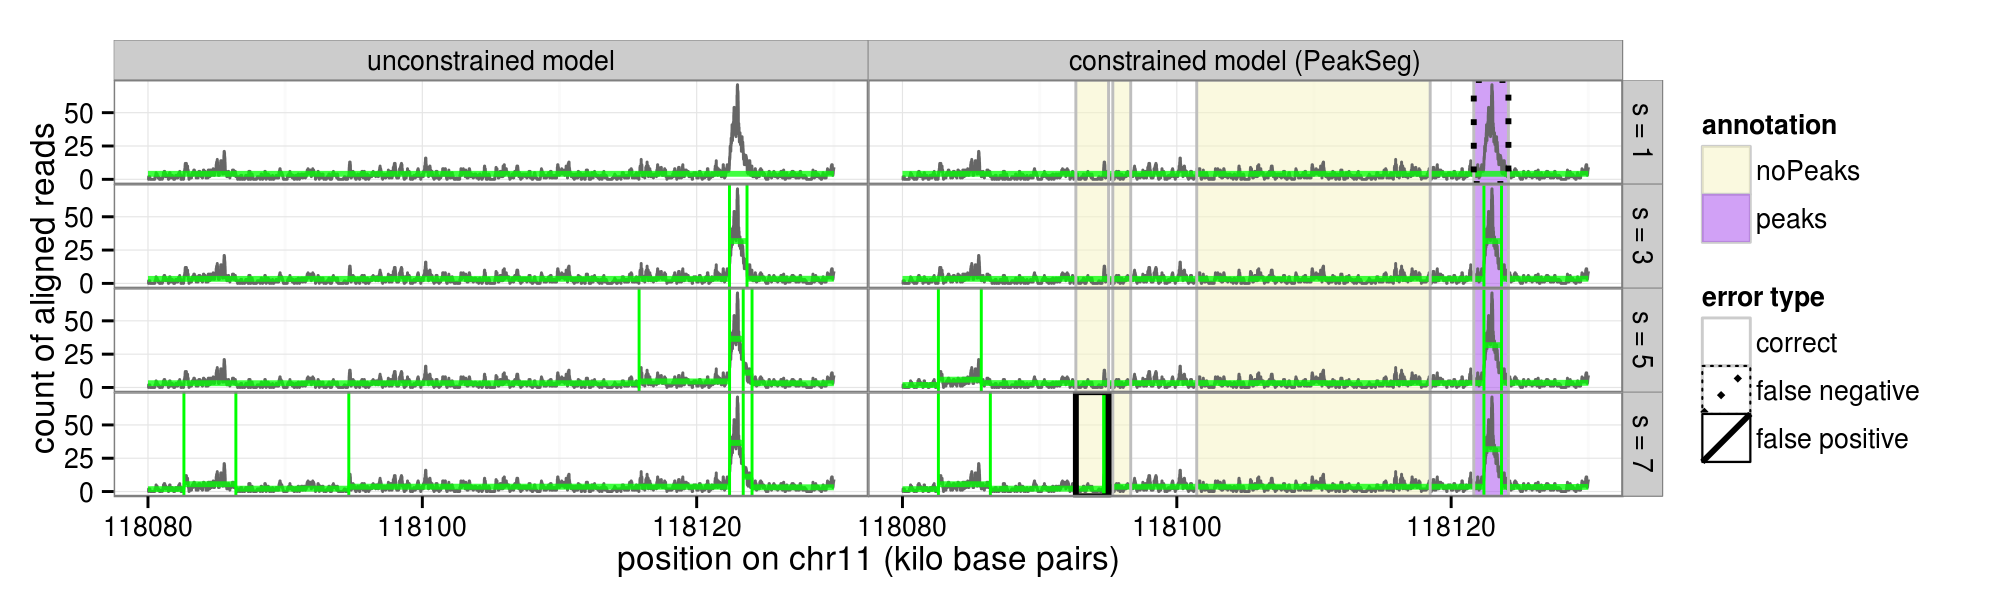
\includegraphics[width=1.1\textwidth]{figure-Segmentor-PeakSeg}

  \begin{itemize}
  \item Previous work: unconstrained maximum likelihood mean\\
    for $s$ segments ($s-1$ changes).
  \item This paper: constraint enforces up, down, up, down\\ (and not
    up, up, down).
  \item Odd-numbered segments are background noise,\\
    even-numbered segments are peaks.
  \end{itemize}
\end{frame}

\begin{frame}[fragile]
  \frametitle{PeakSeg:  constrained maximum likelihood
    segmentation}
For each number of segments $s\in\{1, \dots,
  s_{\text{max}}\}$,\\
the PeakSeg model for the mean vector $\mathbf m$ is defined as:

  \begin{eqnarray*}
  \label{PeakSeg}
  \mathbf{\tilde m}^s(\mathbf y)  =
    \argmin_{\mathbf m\in\RR^{d}}& &\ \ 
\sum_{j=1}^d
      %\log\Lik(y_{j}, m_{j})
      m_j - y_j \log m_j\text{ (PoissonLoss)}
      %\rho(\mathbf m, \mathbf y) 
\\
    \text{such that}& &\ \  \Segments(\mathbf m)=s,  \\
    \alert<1>{\forall j\in\{1, \dots, d\},} & &
    \ \ \alert<1>{P_j(\mathbf m) \in\{0, 1\}.}\\
    && \alert<1>{\text{up, down, up, down constraint.}}
   \end{eqnarray*}
where the peak indicator $P_1(\mathbf m)=0$ and for $j>1$,
\begin{equation*}
  \label{eq:peaks}
  P_j(\mathbf m) = \sum_{k=2}^j \sign( m_{k} - m_{k-1} ).
\end{equation*}

We propose cDPA = a constrained dynamic programming algorithm, which
computes $s_{\text{max}}$ models in $O(s_{\text{max}} d^2)$ time.

\end{frame}

% \begin{frame}
%   \frametitle{Previous work on breakpoint detection}
%   G Rigaill, TD Hocking, \emph{et al.} Learning Sparse Penalties for Change
%   Point Detection using Max Margin Interval Regression, ICML 2013.
%   \begin{itemize}
%   \item Supervised algorithm for detecting change points in piecewise
%     constant DNA copy number profiles.
%   \item Inputs: genomic profile $\mathbf y$, \\
%     profile features $\mathbf x$, \\
%     manually annotated regions $R$ (change point locations).
%   \item Method: compute maximum likelihood segmentations $\mathbf{\hat
%       m}^1(\mathbf y), \dots, \mathbf{\hat m}^{s_{\text{max}}}(\mathbf
%     y)$, learn a penalty function $f(\mathbf x) \Rightarrow \hat s$
%     that minimizes the number of incorrect regions $R$.
%     \item Output: the segmentation with minimum predicted error
%       $\mathbf{\hat m}^{\hat s}(\mathbf y)$.
%   \end{itemize}
%   We can use the same method for peak detection!
% \end{frame}

\section{Train and test error results, conclusions}

\begin{frame}
  \frametitle{Train error on H3K4me3 data}
  \includegraphics[width=\textwidth]{figure-dp-peaks-train-1}
\end{frame}

\begin{frame}
  \frametitle{Train error on H3K36me3 data}
  \includegraphics[width=\textwidth]{figure-dp-peaks-train-2}
\end{frame}

\begin{frame}
  \frametitle{AIC/BIC and oracle penalty function learning}

Supervised learning method of Hocking, Rigaill, et al (ICML 2013).\\
Oracle model complexity of Cleynen and Lebarbier (2014).\\

Predicted number of segments for each profile $i$:

\begin{equation*}
  \hat s_i = 
  \argmin_{s}
  \text{PoissonLoss}\left[
    \mathbf{\tilde m}^s(\mathbf y_i),
    \mathbf y_i
  \right]
  + 
  \overbrace{
    \underbrace{\alert<1>{h(p, d_i)}}_{\text{given}}
    \underbrace{\alert<2>{\lambda_i}}_{\text{learned}}
  }^{\text{penalty}},
\end{equation*}

  Names: (model complexity).(number of parameters learned):

  \begin{center}
  \begin{tabular}{ll}
    \textbf{name} & \textbf{model complexity} \alert<1>{$h(s, d_i)$} \\
    \hline
    AIC/BIC.* & \alert<1>{$s$}\\
    oracle.* & \alert<1>{$s\left(1 + 4\sqrt{1.1 + \log(d_i/s)}\right)^2$}
  \end{tabular}
\end{center}

  \begin{center}
    \small
  \begin{tabular}{lllll}
    \textbf{name} & \textbf{learned} \alert<2>{$\lambda_i$} & 
    \textbf{parameters} & \textbf{learning algorithm} \\
    \hline
    *.0 & AIC=\alert<2>{2}, BIC=\alert<2>{$\log d_i$} & none & unsupervised \\
    *.1 & 
    \alert<2>{$\beta$} & 
    $\beta\in\RR_+$ & grid search \\
    *.3 & 
    \alert<2>{$e^\beta d_i^{w_1} (\max \mathbf y_i)^{w_{2}}$} & 
    $\beta, w_1, w_{2}\in\RR$ & interval regression \\
    *.41 & 
    \alert<2>{$\exp(\beta + \mathbf w^\intercal \mathbf x_i)$} & 
    $\beta\in\RR, \mathbf w\in\RR^{40}$ & 
    regularized int. reg. \\
  \end{tabular}
\end{center}


\end{frame}

\begin{frame}
  \frametitle{Unsupervised constrained optimization algorithm works
    for both H3K36me3 and H3K4me3 data types}

  ...except in the H3K4me3\_XJ\_immune data set.

  \includegraphics[width=\textwidth]{figure-dp-peaks-regression-dots-unsupervised}
  
  Six train/test splits (open circles) and mean (shaded circle).
\end{frame}

\begin{frame}
  \frametitle{Training 1 parameter with grid search reduces test error}

  ...except for macs, good defaults for 3/4 H3K4me3 data sets.

  \includegraphics[width=\textwidth]{figure-dp-peaks-regression-dots-grid}

  Six train/test splits (open circles) and mean (shaded circle).
\end{frame}

\begin{frame}
  \frametitle{Training several parameters with interval regression 
    further reduces test error}

  ...except when there are few train data (H3K36me3\_TDH).

  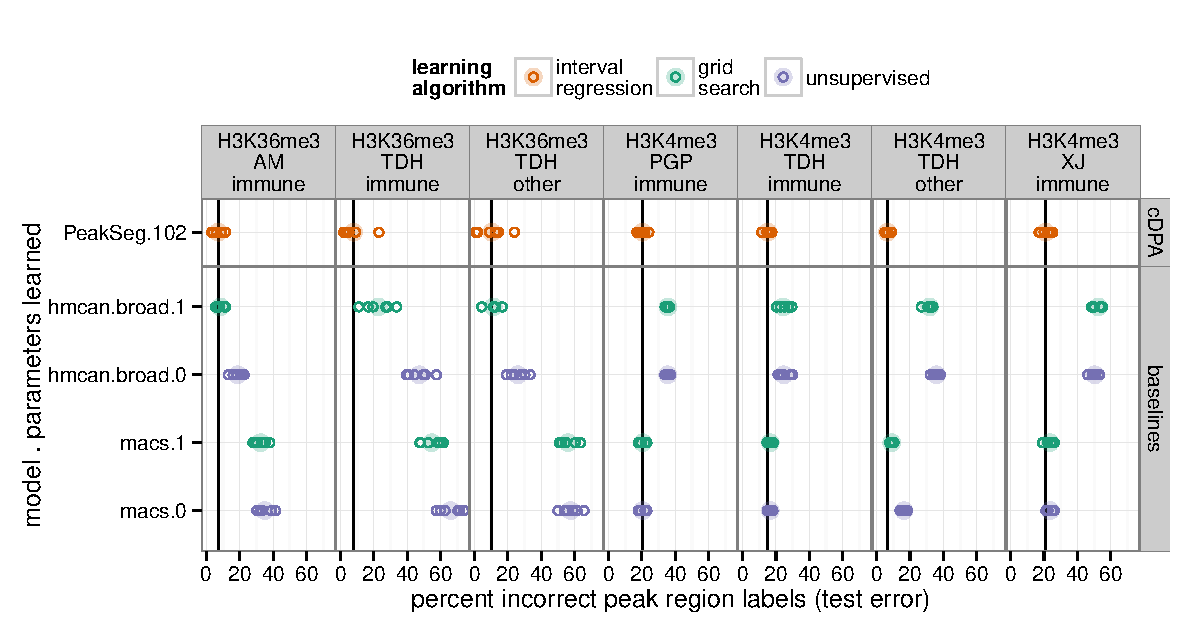
\includegraphics[width=\textwidth]{figure-dp-peaks-regression-dots}

  Six train/test splits (open circles) and mean (shaded circle).
\end{frame}

\begin{frame}
  \frametitle{Conclusions and future work}
  PeakSeg: \textbf{Peak} detection via constrained optimal
  \textbf{Seg}mentation.
  \begin{itemize}
  \item New segmentation model with up, down, up, down constraint.
  \item First supervised peak detection algorithm.
  \item State-of-the-art peak detection for both H3K4me3 and H3K36me3
    profiles.
  \item Oracle model complexity more accurate
    than AIC/BIC.
  \end{itemize}
  Future work:
  \begin{itemize}
  \item Constrained version of Pruned Dynamic Programming (Rigaill
    arXiv:1004.0887) to compute in $O(d\log d)$ time.
  \item Efficient algorithm which provably computes PeakSeg model?
  \item Theoretically optimal features for the penalty learning
    problem?
  \item Feature learning based on profile count data.
  \item Overlapping peaks at the same positions across samples
    (arXiv:1506.01286).
  \end{itemize}
\end{frame}

\begin{frame}
  \frametitle{Thanks for your attention!}
  Write me at \alert{\texttt{toby.hocking@mail.mcgill.ca}} to collaborate!

  \vskip 1cm

  Source code for slides, figures, paper online!\\
  \small
  \url{https://github.com/tdhock/PeakSeg-paper}
  \vskip 1cm

  Supplementary slides appear after this one.

\end{frame}

\begin{frame}
  \frametitle{PeakSeg accuracy can be quantified using labels}
  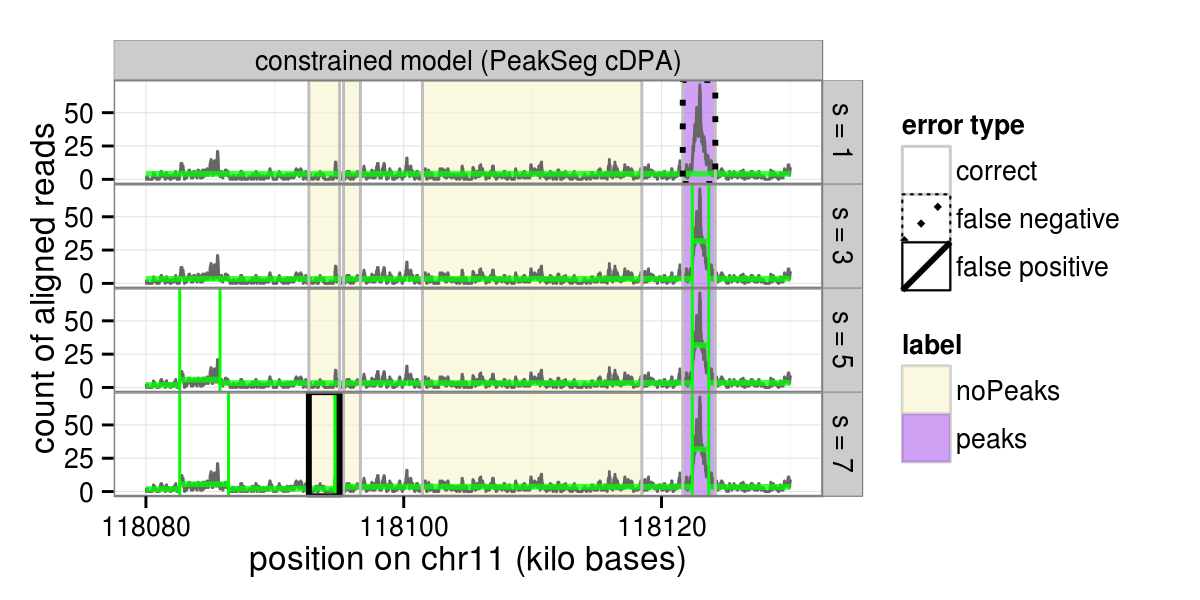
\includegraphics[width=\textwidth]{figure-Segmentor-PeakSeg-constrained-regions}

  \begin{itemize}
  \item $1, 3, 5, 7$ segments = $0, 1, 2, 3$ peaks ($2p + 1 = s$).
  \item Models with $s\in\{1, 7\}$ segments have 1 incorrect region.
  \item Models with $s\in\{3, 5\}$ segments are perfect.
  \item Goal for $i\in\{1, \dots, n\}$ profiles:\\
    predict profile-specific segments $\hat s_i$ with minimum errors.
  \end{itemize}
\end{frame}

\begin{frame}
  \frametitle{Chromatin immunoprecipitation sequencing (ChIP-seq)}
  Analysis of DNA-protein interactions.

  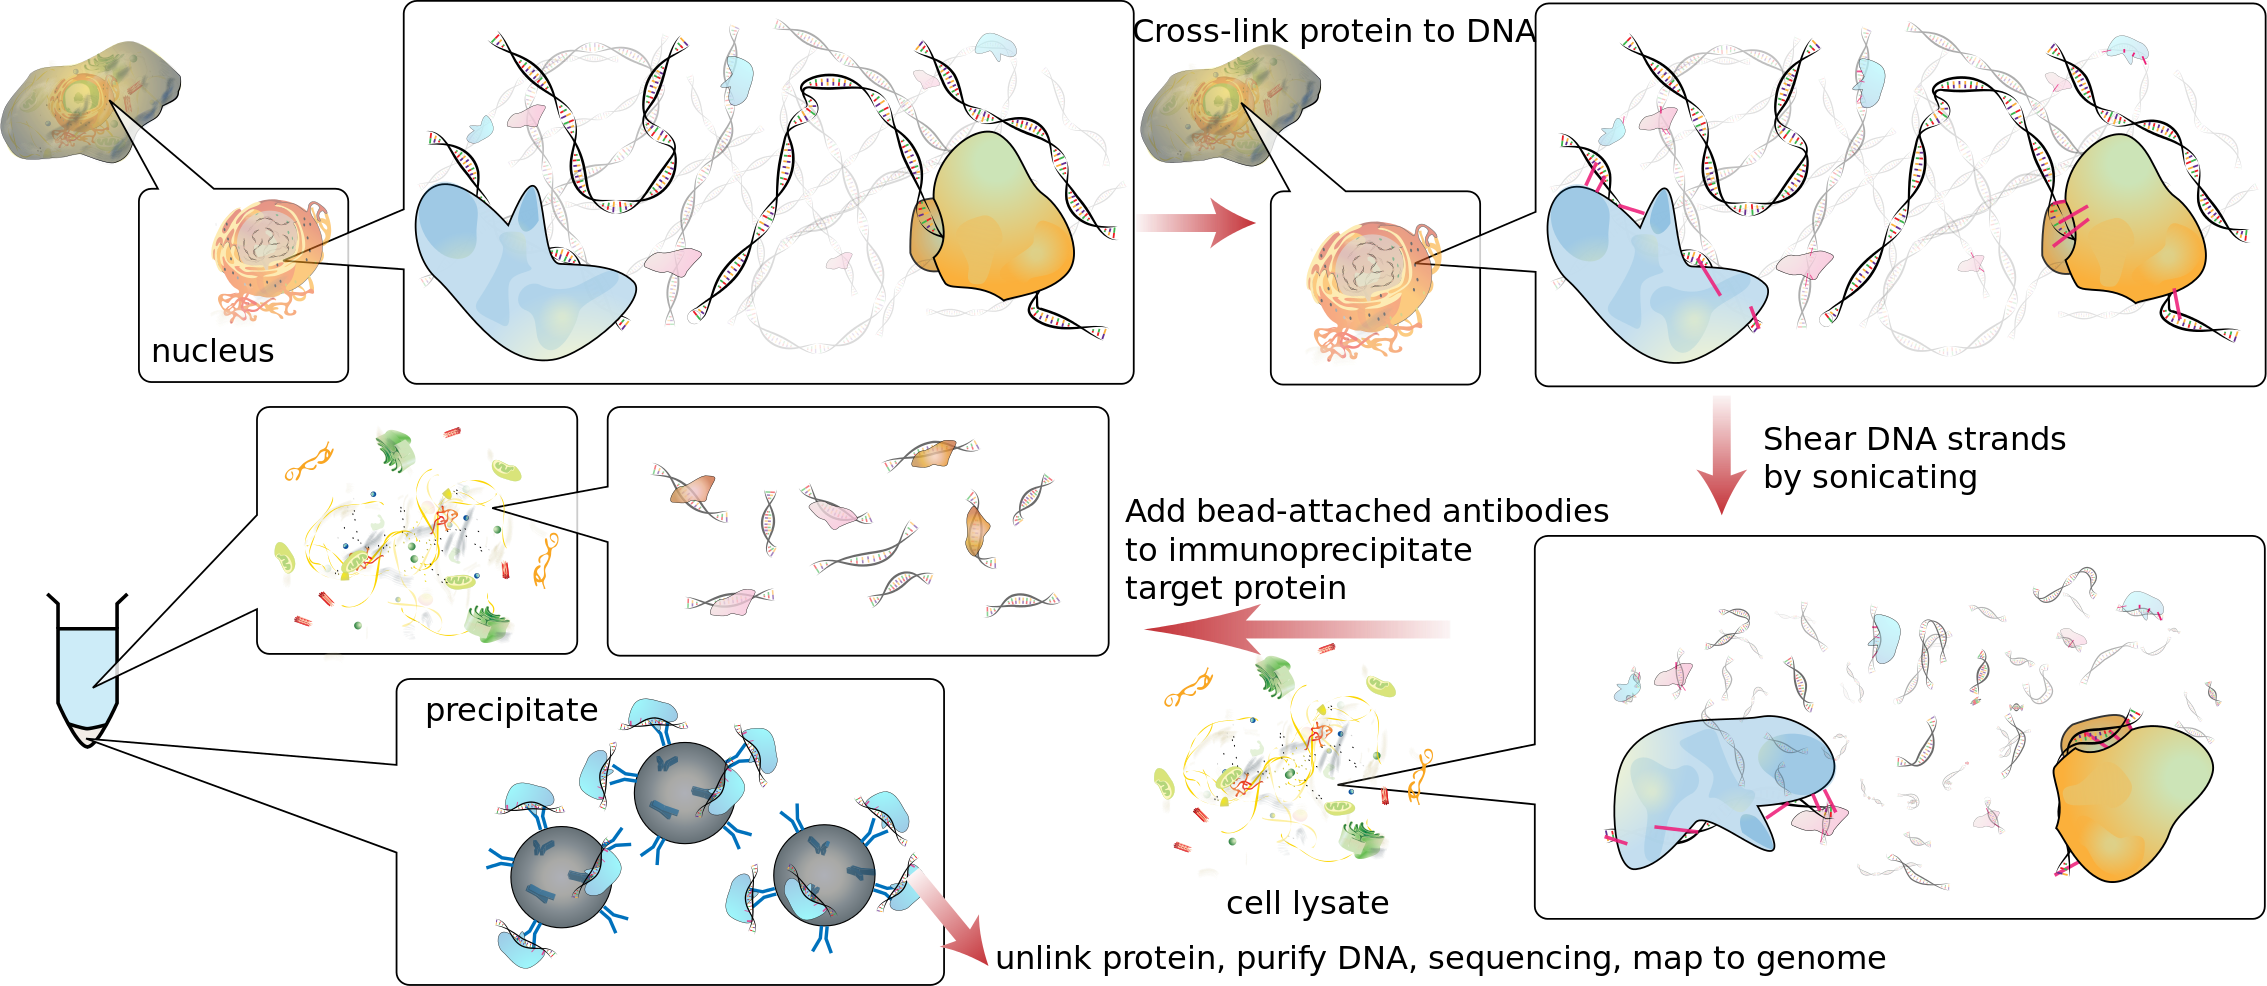
\includegraphics[width=\textwidth]{Chromatin_immunoprecipitation_sequencing_wide.png}

  Source: ``ChIP-sequencing,'' Wikipedia.
\end{frame}

\begin{frame}
  \frametitle{Previous work in computer vision: look and add labels
    to...}
  \begin{tabular}{ccc}
    Photos & Cell images & Copy number profiles \\
    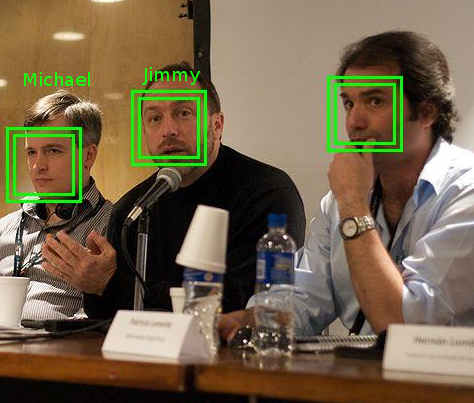
\includegraphics[width=1.3in]{faces} &
    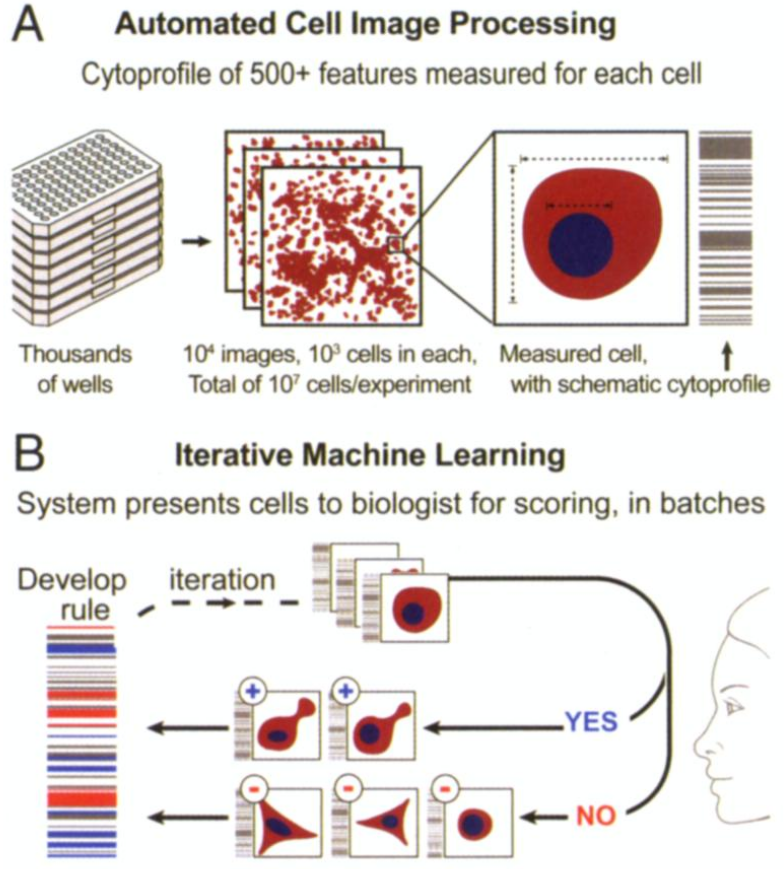
\includegraphics[width=1.3in]{cellprofiler} &
    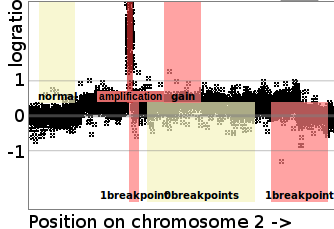
\includegraphics[width=1.5in]{regions-axes}\\
    Labels: names & phenotypes & alterations \\ \\
    CVPR 2013 & CellProfiler & SegAnnDB \\
    246 papers & 873 citations & H, \emph{et. al.} 2014. \\
     &
  \end{tabular}
  Sources: \url{http://en.wikipedia.org/wiki/Face_detection}\\
  Jones et al PNAS 2009. Scoring diverse cellular morphologies in
  image-based screens with iterative feedback and machine learning.
\end{frame}


\input{figure-dp-first}

\input{figure-dp-short}

\input{figure-dp}

\begin{frame}
  \frametitle{Dynamic programming is faster than grid search for $s>
    2$ segments}

  Computation time in number of data points $d$:

  \vskip 1cm

  \begin{tabular}{ccc}
    segments $s$ & grid search & dynamic programming \\
    \hline
    1 & $O(d)$ & $O(d)$ \\
    2 & $O(d^2)$ & $O(d^2)$ \\
    3 & $O(d^3)$ & $O(d^2)$ \\
    4 & $O(d^4)$ & $O(d^2)$ \\
    $\vdots$ &     $\vdots$ &     $\vdots$ 
  \end{tabular}

  \vskip 1cm

  For example $d = 5735$ data points to segment.\\
  $d^2 = 32890225$\\
  $d^3 = 188625440375$\\
  $\vdots$
\end{frame}

\input{figure-dp-third}

\begin{frame}
  \frametitle{Step 1: compute annotation error functions}
  \begin{itemize}
  \item Inputs: for $i\in\{1, \dots, n\}$ samples, genomic profiles
    $\mathbf y_i$, annotated regions $R_i$.
    \begin{equation*}
      \begin{array}{cccc}
        & \text{0 peaks} & \cdots & \text{$p_{\text{max}}$ peaks}\\
        \hline
        \text{segmentations} &
        \mathbf{\tilde m}^0(\mathbf y_i) & 
        \cdots & 
        \mathbf{\tilde m}^{p_{\text{max}}}(\mathbf y_i)\\
        \text{annotation error} & 
        e_i(0) &
        \cdots & 
        e_i(p_{\text{max}})\\
      \end{array}
    \end{equation*}
  \item R package \url{https://github.com/tdhock/PeakError/} computes
    the \textbf{annotation error}
    $e_i:\{0,\dots,p_{\text{max}}\}\rightarrow \ZZ_+$.
  \item   TD Hocking \emph{et al.} Visual annotations and a supervised
    learning approach for evaluating and calibrating ChIP-seq peak detectors
    (arXiv:1409.6209).
  \end{itemize}
\end{frame}

\begin{frame}
  \frametitle{Step 2: compute model selection functions}
  For each sample/chromosome $i\in\{1, \dots, n\}$, for $\lambda\in\RR_+$,
  \begin{itemize}
  \item   The \textbf{optimal number of peaks} function is
  \begin{equation*}
    p_i^*(\lambda) = \argmin_{p\in\{1,\dots, p_{\text{max}}\}}
      \alpha_i^p + \lambda p,
  \end{equation*}
  where  $\alpha_i^p$ is the Poisson loss of the model with $p$ peaks.
  % \begin{equation*}
  %   \label{eq:loss}
  %   L_i^p = \sum_{j=1}^d \tilde m^p_{ij} - y_{ij} \log \tilde m^p_{ij}.
  % \end{equation*}
  \item The \textbf{penalized annotation error} function is
  \begin{equation*}
    E_i(\lambda) = e_i\left[ p_i^*(\lambda) \right],
  \end{equation*}
  where $e_i(p)$ is the number of incorrect annotations for the model
  with $p$ peaks.
  \end{itemize}
  \textbf{Peaks $p_i^*$ and error $E_i$ are non-convex, piecewise
    constant functions that can be computed exactly.}
\end{frame}
 
\begin{frame}
  \frametitle{Step 3: learn a penalty function via interval regression}
  \begin{itemize}
  \item Compute the target interval $(\underline L_i, \overline
    L_i)$.
  \item $\log \lambda_i\in(\underline L_i, \overline L_i) \Rightarrow$
   optimal peak detection.
  \item Compute simple features $\mathbf x_i\in\RR^m$, e.g. chromosome size,
    read counts, signal scale $\log \max \mathbf y_i $.
  \item Learn an optimal affine $f(\mathbf x_i) =
    \beta + \mathbf w^\intercal \mathbf x_i = \log \lambda_i $.
    % \begin{equation*}
    %   \minimize_{\beta\in\RR, \mathbf w\in\RR^m} \sum_{i=1}^n \ell\left[
    %     (\underline L_i, \overline L_i),
    %     \beta + \mathbf w^\intercal \mathbf x_i 
    %   \right]
    %   + ||w||_1.
    % \end{equation*}
  \item Equivalent to learning a penalty $\lambda_i = \exp
    f(\mathbf x_i)$:
    \begin{eqnarray*}
  p_i^*[\exp f(\mathbf x_i)] 
&=& \argmin_p  \alpha_i^p +  p \exp f(\mathbf x_i) \\
&=& \argmin_p \alpha_i^p + p (\max \mathbf y_i)^w e^\beta.
\end{eqnarray*}
  \item Convex optimization problem, global optimum, variable
    selection (G Rigaill, TD Hocking, \emph{et al.} ICML 2013).
  \end{itemize}
\end{frame}

\begin{frame}
  \frametitle{Summary of supervised PeakSeg 
     algorithm}
  \begin{itemize}
  \item Fix the maximum number of peaks $p_{\text{max}} = 10,000$.
  \item For each sample/chromosome $i\in\{1,\dots, n\}$,
    \begin{itemize}
    \item \textbf{Unsupervised PeakSeg}: compute constrained maximum likelihood
      segmentations $\mathbf{\tilde m}^0(\mathbf y_i), \dots,
      \mathbf{\tilde m}^{p_{\text{max}}}(\mathbf y_i)$.
    \item Step 1: use annotated region labels to compute the
      annotation error $e_i(0), \dots, e_i(p_{\text{max}})$.
    \item Step 2: compute peaks $p_i^*(\lambda)$, error
      $E_i(\lambda)$, and target interval $(\underline L_i, \overline
      L_i)$.
    \end{itemize}
  \item  Step 3:  learn a  penalty $\lambda_i  = \exp  f(\mathbf x_i)$
    using features $\mathbf x_i$ such as $\log \max(\mathbf y_i)$.
  \item Given an unlabeled chromosome $(\mathbf x, \mathbf y)$, we predict
    $\mathbf{ \tilde m}^{p^*\left[
        \exp f(\mathbf x)
      \right]}(\mathbf y)$.
  %\item Optional post-processing: mean of overlapping peaks.
  \end{itemize}
\end{frame}

\begin{frame}
  \frametitle{Benchmark: 7 annotated region data sets}
  \url{http://cbio.ensmp.fr/~thocking/chip-seq-chunk-db/}
  \begin{itemize}
  \item 4 annotators (AM, TDH, PGP, XJ).
  \item 8 cell types.
  \item 37 annotated H3K4me3 profiles (sharp peaks).
  \item 29 annotated H3K36me3 profiles (broadly enriched domains).
  \item 12,826 annotated regions in total.
  \item 2752 separate segmentation problems.
  \end{itemize}
  Used the cDPA on the annotated data.
  \begin{itemize}
  \item cDPA computed models with $0, \dots, 9$ peaks\\
    (for 99.5\% of problems).
  \item For the biggest problem, cDPA took 3 hours.\\
    ($d=88,509$ data points, 3.5 megabases)
  \item macs takes about 90 minutes for one whole genome.
  \end{itemize}
\end{frame}

\begin{frame}
  \frametitle{Maximum likelihood segmentations}
  For a coverage profile $\mathbf y\in\ZZ_+^d$,
  find the mean vector $\mathbf{\hat m}^s(\mathbf y)\in\RR^d$ with
  maximum Poisson likelihood, given $s$ segments ($s-1$ change-points).

  \includegraphics[width=\textwidth]{figure-Segmentor-PeakSeg-unconstrained}

  Computed via Segmentor3IsBack R package (Cleynen et al. 2014)

\end{frame}

\begin{frame}
  \frametitle{Previous work: maximum likelihood segmentation}
  \begin{itemize}
  \item   Let $\mathbf y = 
\left[
  \begin{array}{ccc}
    y_1 & \cdots & y_d
  \end{array}
\right]
\in\ZZ_+^d$ be the aligned read counts for one sample
  and one genomic region.
%\item For example the biggest chromosome in hg19 (chr1) has
%  $d=249,250,621$ bases.
\item Fix $s_{\text{max}}=19$, the maximum number of segments.
\item For each number of segments $s\in\{1, \dots,
  s_{\text{max}}\}$, we want:
  \end{itemize}
  \begin{equation*}
    \label{argmax:M}
    \begin{aligned}
      \mathbf{\hat m}^s(\mathbf y)  =\ 
      &\argmin_{\mathbf m\in\RR^{d}} && \sum_{j=1}^d
      %\log\Lik(y_{j}, m_{j})
      m_j - y_j \log m_j \text{ (Poisson loss)}
      \\
      \\
      &\text{such that} && \Segments(\mathbf m)=s.
    \end{aligned}
  \end{equation*}
  \begin{itemize}
  \item Pruned Dynamic Programming (Rigaill arXiv:1004.0887) returns
    $\mathbf{\hat m}^1(\mathbf y), \dots, \mathbf{\hat
      m}^{s_{\text{max}}}(\mathbf y)$ in $O(s_{\text{max}} d\log d)$
    time.
  \end{itemize}
\end{frame}

\begin{frame}
  \frametitle{Maximum likelihood segmentations}
  \includegraphics[width=\textwidth]{figure-Segmentor-PeakSeg-unconstrained}
  
  Model with $s=5$ segments changes up, up, down, down.\\
  How to define peaks? Introduce a threshold parameter?
\end{frame}

\begin{frame}
  \frametitle{Constrained maximum likelihood segmentations}
  \includegraphics[width=\textwidth]{figure-Segmentor-PeakSeg-constrained}

  Model with $s=5$ segments changes up, down, up, down.\\
  Peaks are even-numbered segments.
\end{frame}

\begin{frame}
  \frametitle{Two annotators provide consistent labels, but different
    precision}
  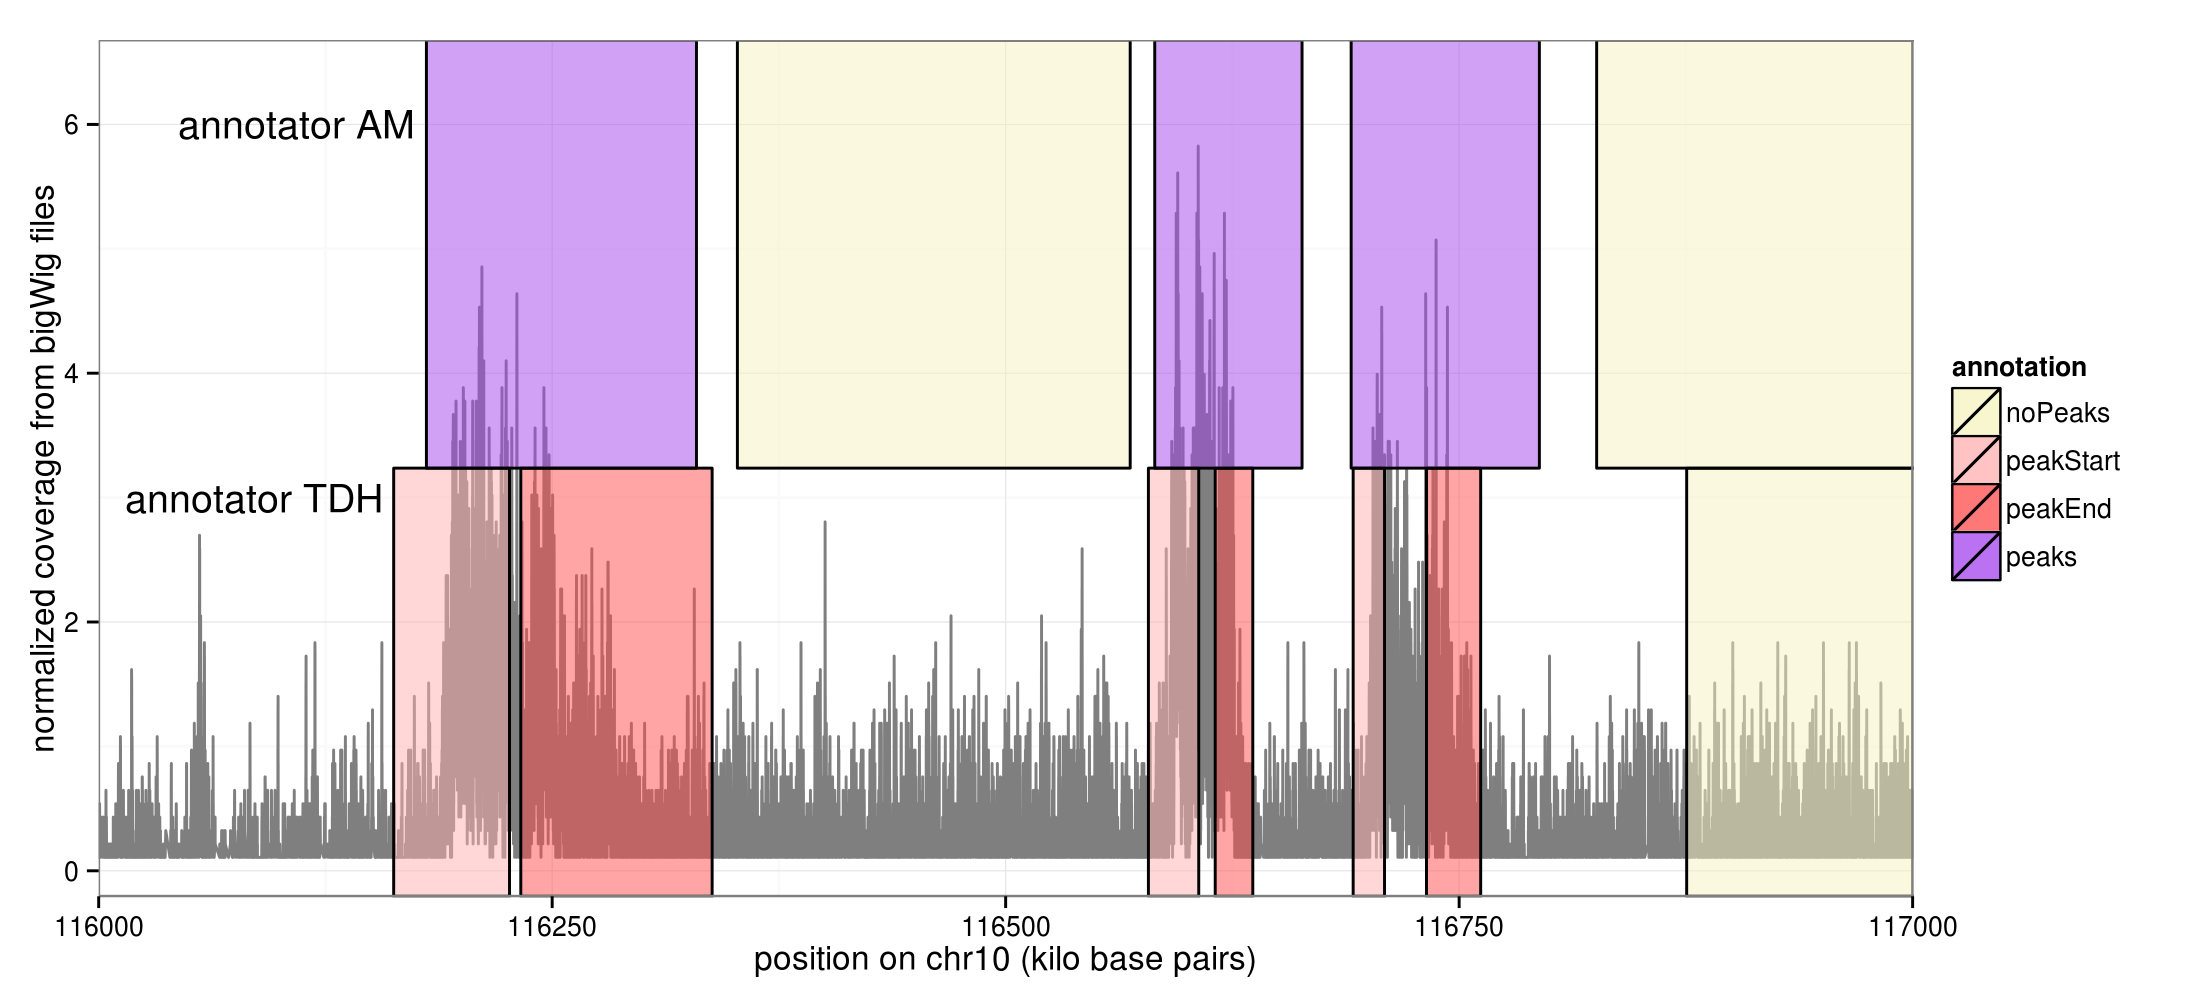
\includegraphics[width=1.1\textwidth]{figure-several-annotators}

  \begin{itemize}
  \item TDH peakStart/peakEnd more precise than AM peaks.
  \item AM noPeaks more precise than TDH no label.
  \end{itemize}
\end{frame}

\begin{frame}
  \frametitle{Comparison on annotated McGill benchmark data set}
  Hocking et al, 2014, arXiv:1409.6209.\\
  \begin{itemize}
  \item Manually annotate regions with or without peaks.\\
    \url{http://cbio.ensmp.fr/~thocking/chip-seq-chunk-db/}
  \item Tune 1 parameter that affects the number of peaks.
  \item Choose the parameter that minimizes the annotation error.
  \end{itemize}
  Results:
  \begin{itemize}
  \item MACS best for H3K4me3 (sharp peak pattern),
  \item HMCan.broad best for H3K36me3 (broad peak pattern).
  \item Consistent across 4 annotators (PhD students, postdocs).
  \item 10--20\% test error rates.
  \end{itemize}
\end{frame}

\begin{frame}
  \frametitle{Can we do better than unsupervised peak detectors? Yes!}
  We propose \textbf{PeakSeg}, a new model with efficient algorithms
  for supervised peak detection.
  \begin{itemize}
  \item Input: \alert<1>{several ChIP-seq profiles},
    \alert<2>{manually annotated regions}.
  \item New methods for peak detection: 
    \begin{itemize}
    \item \alert<1>{Constrained optimal segmentation}.
    \item Efficient \alert<2>{supervised learning using manually annotated
      regions}.
    \end{itemize}
  \item Output: predicted peaks for each profile.
  %\item and consistent peak boundaries across samples.
  \end{itemize}
  State-of-the-art peak detection accuracy (on both sharp H3K4me3 and
  broad H3K36me3 profiles).
\end{frame}

\begin{frame}
  \frametitle{Existing peak detection algorithms}
  \begin{itemize}
  \item Model-based analysis of ChIP-Seq (MACS), Zhang et al, 2008.
  \item SICER, Zang et al, 2009.
  \item HOMER findPeaks, Heinz et al, 2010.
  \item RSEG, Song and Smith, 2011.
  \item Histone modifications in cancer (HMCan), Ashoor et al, 2013.
  \item ... dozens of others.
  \end{itemize}
  Two big questions: how to choose the best...
  \begin{itemize}
  \item ...algorithm?
  \item ...parameters?
  \end{itemize}
\end{frame}

\begin{frame}[fragile]
  \frametitle{How to choose model parameters?}
\scriptsize
19 parameters for Model-based analysis of ChIP-Seq (MACS), Zhang et al, 2008.
\begin{verbatim}
  [-g GSIZE]
  [-s TSIZE] [--bw BW] [-m MFOLD MFOLD] [--fix-bimodal]
  [--nomodel] [--extsize EXTSIZE | --shiftsize SHIFTSIZE]
  [-q QVALUE | -p PVALUE | -F FOLDENRICHMENT] [--to-large]
  [--down-sample] [--seed SEED] [--nolambda]
  [--slocal SMALLLOCAL] [--llocal LARGELOCAL]
  [--shift-control] [--half-ext] [--broad]
  [--broad-cutoff BROADCUTOFF] [--call-summits]
\end{verbatim}
10 parameters for Histone modifications in cancer (HMCan),
Ashoor et al, 2013.
\begin{verbatim}
minLength 145
medLength 150
maxLength 155
smallBinLength 50
largeBinLength 100000
pvalueThreshold 0.01
mergeDistance 200
iterationThreshold 5
finalThreshold 0
maxIter 20
\end{verbatim}
\end{frame}

\end{document}
